% =====================================================================
%  SLIDE BÁO CÁO PROJECT II – ĐỀ TÀI 1A (Beamer, 16:9)
%  Biên dịch: latexmk -xelatex slides.tex
% =====================================================================
\documentclass[aspectratio=169,11pt]{beamer}

\usepackage{fontspec}
\usepackage{polyglossia}
\setdefaultlanguage{vietnamese}
\setsansfont{Arial}
\setmonofont[Scale=0.85]{Consolas}

\usepackage{graphicx}
\usepackage{booktabs,tabularx,array}
\usepackage[table]{xcolor}
\usepackage{listings}
\usepackage{tikz}
\graphicspath{{../report/images/}{../report/images/screens/}{../docs/diagrams/png/}}

% ---------- Màu nhận diện (đỏ Bách Khoa + xanh navy)
\definecolor{hustred}{HTML}{B3261E}
\definecolor{navy}{HTML}{14213D}
\definecolor{blueA}{HTML}{1F4E8C}
\definecolor{soft}{HTML}{F4F6FA}
\definecolor{okgreen}{HTML}{1E7B45}
\definecolor{warn}{HTML}{A15C00}

\usetheme{Madrid}
\usecolortheme{whale}
\setbeamercolor{palette primary}{bg=navy,fg=white}
\setbeamercolor{palette secondary}{bg=blueA,fg=white}
\setbeamercolor{palette tertiary}{bg=hustred,fg=white}
\setbeamercolor{titlelike}{parent=palette primary}
\setbeamercolor{structure}{fg=navy}
\setbeamercolor{frametitle}{bg=navy,fg=white}
\setbeamercolor{block title}{bg=navy,fg=white}
\setbeamercolor{block body}{bg=soft,fg=black}
\setbeamercolor{block title alerted}{bg=hustred,fg=white}
\setbeamercolor{block body alerted}{bg=hustred!6,fg=black}
\setbeamercolor{block title example}{bg=okgreen,fg=white}
\setbeamercolor{block body example}{bg=okgreen!7,fg=black}
\setbeamercolor{item}{fg=hustred}
\setbeamercolor{alerted text}{fg=hustred}
\setbeamertemplate{navigation symbols}{}
\setbeamertemplate{itemize items}[circle]
\setbeamertemplate{blocks}[rounded][shadow=false]
\setbeamerfont{frametitle}{size=\large,series=\bfseries}
\setbeamertemplate{caption}{\raggedright\insertcaption\par}

% Chân trang: tên ngắn | mục | số trang
\setbeamertemplate{footline}{%
  \leavevmode\hbox{%
  \begin{beamercolorbox}[wd=.38\paperwidth,ht=2.4ex,dp=1ex,left]{palette primary}\hspace*{2ex}\usebeamerfont{author in head/foot}Project II – Đề tài 1A · Nguyễn Lê Quân\end{beamercolorbox}%
  \begin{beamercolorbox}[wd=.46\paperwidth,ht=2.4ex,dp=1ex,center]{palette secondary}\usebeamerfont{title in head/foot}\insertsectionhead\end{beamercolorbox}%
  \begin{beamercolorbox}[wd=.16\paperwidth,ht=2.4ex,dp=1ex,right]{palette tertiary}\insertframenumber{} / \inserttotalframenumber\hspace*{2ex}\end{beamercolorbox}}%
  \vskip0pt}

\lstdefinelanguage{JavaScript}{
  keywords={const,let,function,return,if,else,for,of,new,throw,true,false,null},
  sensitive=true, comment=[l]{//}, morestring=[b]', morestring=[b]"}
\lstset{language=JavaScript, basicstyle=\ttfamily\scriptsize, keywordstyle=\color{hustred}\bfseries,
  commentstyle=\color{black!55}\itshape, stringstyle=\color{okgreen}, backgroundcolor=\color{soft},
  frame=single, rulecolor=\color{black!15}, columns=fullflexible, keepspaces=true, showstringspaces=false,
  breaklines=true, texcl=true, xleftmargin=4pt, framesep=4pt}

\newcommand{\hd}[1]{\textbf{\color{white}#1}}
\newcommand{\headrow}{\rowcolor{navy}}
\newcommand{\shot}[2][\linewidth]{{\setlength{\fboxsep}{0pt}\color{black!25}\fbox{\includegraphics[width=#1]{#2}}}}
\renewcommand{\arraystretch}{1.2}
\arrayrulecolor{black!45}

\title[Quản lý trung tâm ngoại ngữ]{Phân tích và thiết kế hệ thống hỗ trợ quản lý\\ trung tâm luyện thi chứng chỉ ngoại ngữ}
\subtitle{Báo cáo Project II – Đề tài 1A}
\author{Nguyễn Lê Quân}
\date{Tháng 11 năm 2026}

\AtBeginSection[]{%
  \begin{frame}[plain]
    \begin{tikzpicture}[remember picture,overlay]
      \fill[navy] (current page.south west) rectangle (current page.north east);
      \fill[hustred] ([yshift=-0.9cm]current page.west) rectangle ([xshift=3.2cm,yshift=-1.02cm]current page.west);
      \node[anchor=west,text=white,font=\Huge\bfseries] at ([xshift=1.2cm,yshift=0.2cm]current page.west) {\insertsectionhead};
      \node[anchor=west,text=white!70,font=\large] at ([xshift=1.2cm,yshift=1.3cm]current page.west) {Phần \thesection};
    \end{tikzpicture}
  \end{frame}}

% =====================================================================
\begin{document}

% ---------------------------------------------------------------- Trang tiêu đề
\begin{frame}[plain,t]
  \begin{tikzpicture}[remember picture,overlay]
    \fill[navy] (current page.north west) rectangle ([yshift=-1.25cm]current page.north east);
    \fill[hustred] ([yshift=-1.25cm]current page.north west) rectangle ([yshift=-1.33cm]current page.north east);
    \node[anchor=west,text=white,font=\bfseries] at ([xshift=0.8cm,yshift=-0.42cm]current page.north west) {ĐẠI HỌC BÁCH KHOA HÀ NỘI};
    \node[anchor=west,text=white,font=\small] at ([xshift=0.8cm,yshift=-0.88cm]current page.north west) {TRƯỜNG CÔNG NGHỆ THÔNG TIN VÀ TRUYỀN THÔNG};
    \node[anchor=north east] at ([xshift=-0.9cm,yshift=-1.75cm]current page.north east) {
\includegraphics[height=3.1cm]{hust_logo.png}};
  \end{tikzpicture}\par
  \vspace*{1.95cm}
  \begin{minipage}{0.74\linewidth}
    {\small\bfseries\color{hustred} BÁO CÁO PROJECT II · ĐỀ TÀI 1A}\\[5pt]
    {\Large\bfseries\color{navy} Phân tích và thiết kế hệ thống hỗ trợ quản lý trung tâm luyện thi chứng chỉ ngoại ngữ\par}
    \vspace{3pt}
    {\normalsize\color{black!65} theo chuẩn quốc gia, quốc tế}
  \end{minipage}

  \vspace{0.9cm}
  \begin{tabular}{@{}ll@{}}
    Giảng viên hướng dẫn: & \textbf{TS. Nguyễn Thị Thu Hương} \\
    Sinh viên thực hiện: & \textbf{Nguyễn Lê Quân} – MSSV 20235199 \\
    Lớp: & Khoa học Máy tính 07 – K68 \\
  \end{tabular}

  \vspace{0.35cm}
  {\small\color{black!60} Hà Nội, tháng 11 năm 2026}
\end{frame}

\begin{frame}{Nội dung trình bày}
  \tableofcontents
\end{frame}

% =====================================================================
\section{Bài toán và phân tích đề bài}

\begin{frame}{Bài toán}
  \begin{columns}[T]
    \begin{column}{0.55\linewidth}
      \textbf{Trung tâm luyện thi} IELTS, TOEIC, VSTEP, Cambridge cần phần mềm hỗ trợ:
      \begin{itemize}
        \item Đăng tải thông tin lớp học \textbf{Online / Offline}
        \item \textbf{Phòng chat} tư vấn trực tuyến
        \item Đăng ký → \textbf{thu học phí} → \textbf{kiểm tra đầu vào} → kết quả về văn phòng để xếp lớp
        \item Lập lịch học, phân phòng cho lớp Offline
      \end{itemize}
    \end{column}
    \begin{column}{0.42\linewidth}
      \begin{alertblock}{Ràng buộc sĩ số của đề bài}
        \textbf{Online:} mở lớp khi $\geq 10$ học viên\\[3pt]
        \textbf{Offline:} mở khi $\geq 20$, tối đa 30\\[3pt]
        \textbf{Vượt 30:} việc tách lớp do \textbf{Lãnh đạo trung tâm} quyết định
      \end{alertblock}
    \end{column}
  \end{columns}
  \vspace{6pt}
  \begin{block}{Phải lập trình 4 chức năng}
    \small (1)~Quảng bá lớp học \; (2)~Nhận đăng ký \; (3)~Tra cứu danh sách lớp \; (4)~Chat room tư vấn
  \end{block}
\end{frame}

\begin{frame}{Bóc tách đề bài thành yêu cầu có mã truy vết}
  \small
  \begin{tabularx}{\linewidth}{|>{\raggedright\arraybackslash}p{4.6cm}|>{\raggedright\arraybackslash}X|l|}
    \hline
    \headrow \hd{Câu trong đề bài} & \hd{Yêu cầu hệ thống} & \hd{Mã} \\ \hline
    Đăng tải lớp, phân loại Online/Offline & Danh mục khoá học, lớp học có thuộc tính hình thức & FR-01, 02 \\ \hline
    Phòng chat tư vấn & Chat thời gian thực, hàng đợi, lưu lịch sử & FR-08..10 \\ \hline
    Thu học phí rồi kiểm tra đầu vào & Hồ sơ có vòng đời; chưa nộp phí thì không được thi & BR-01 \\ \hline
    Kết quả về văn phòng để xếp lớp & Quy đổi CEFR, xếp lớp theo trình độ & FR-11, BR-06 \\ \hline
    Offline 20–30, vượt 30 lãnh đạo quyết định & Ngưỡng sĩ số + quy trình tờ trình phê duyệt & BR-03, 04 \\ \hline
    Online không ít hơn 10 & Ngưỡng mở lớp online = 10 & BR-02 \\ \hline
    Lập lịch, phân phòng & Kiểm tra trùng phòng, trùng giảng viên, sức chứa & BR-05, 08 \\ \hline
  \end{tabularx}
  \vspace{6pt}

  \textbf{Kết quả:} 14 yêu cầu chức năng (FR) · 8 quy tắc nghiệp vụ (BR) · 5 tác nhân · 10 use case
\end{frame}

\begin{frame}{Tác nhân và use case tổng quát}
  \begin{columns}[c]
    \begin{column}{0.47\linewidth}
      \centering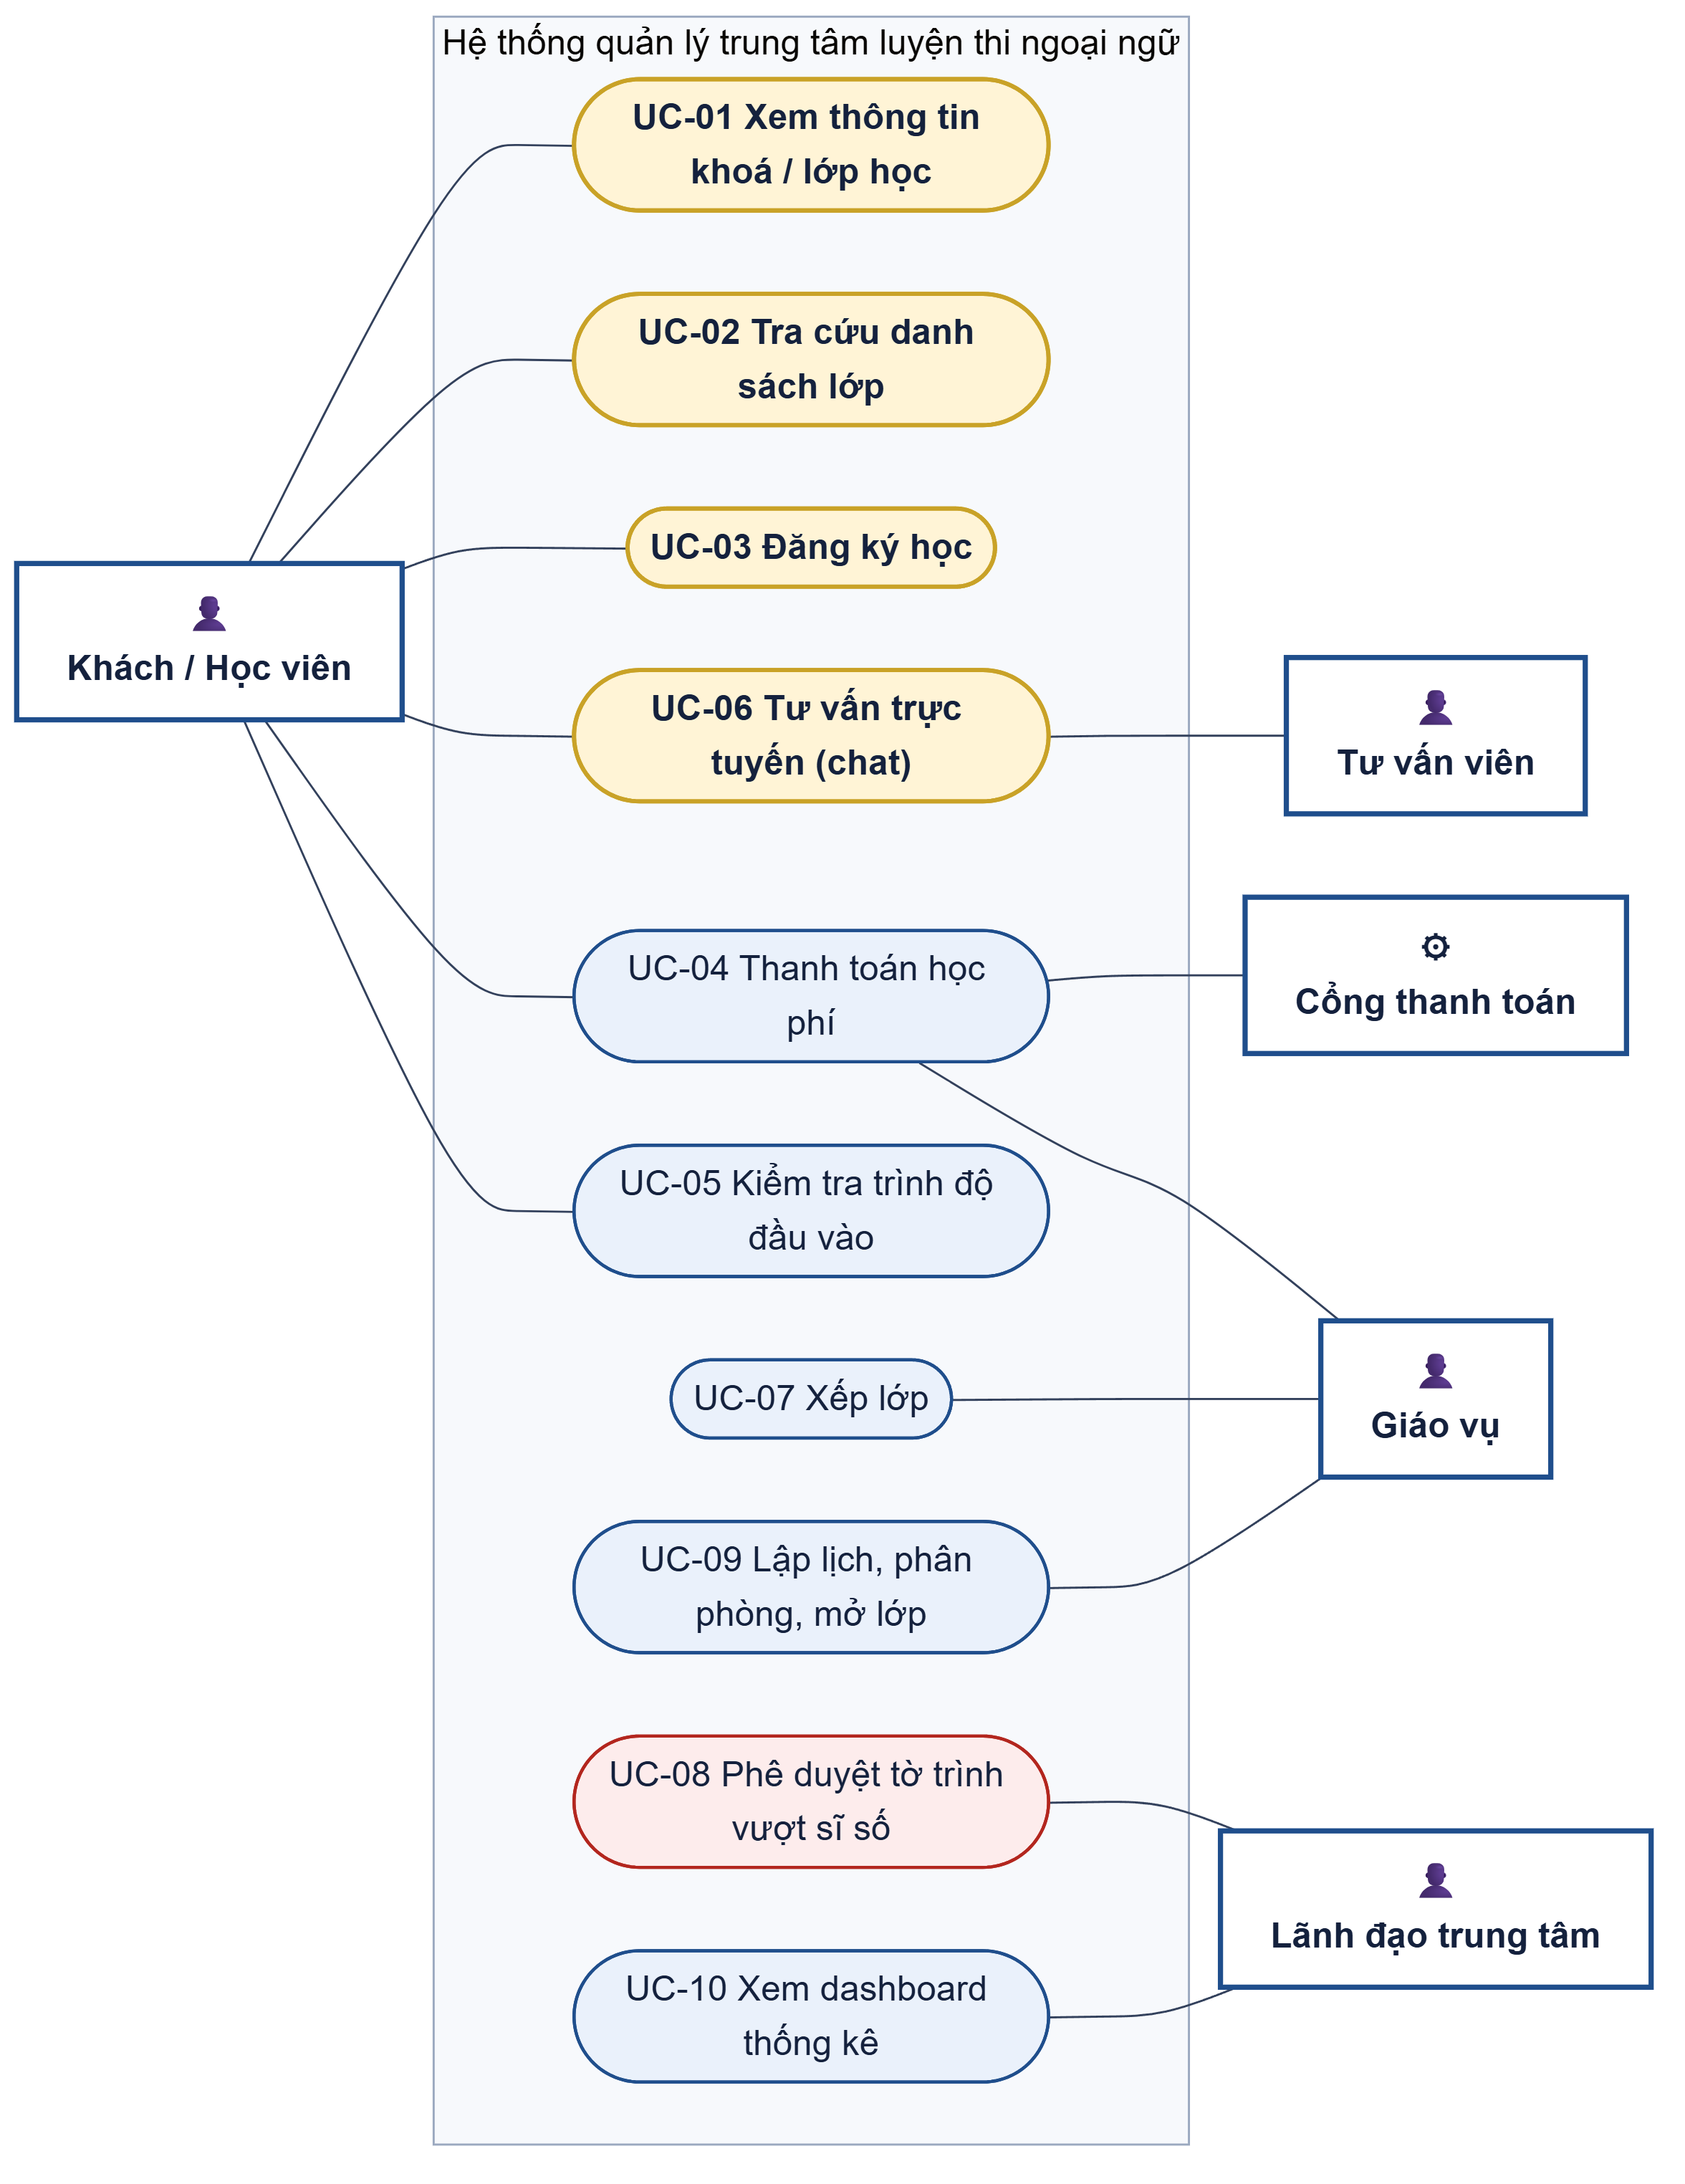
\includegraphics[height=0.80\textheight]{uc_00_tong_quat}
    \end{column}
    \begin{column}{0.5\linewidth}
      \begin{itemize}
        \item \textbf{Khách / Học viên:} xem, tra cứu, đăng ký, nộp phí, làm bài, chat
        \item \textbf{Tư vấn viên:} nhận phiên chat, trả lời
        \item \textbf{Giáo vụ:} xếp lớp, lịch – phòng, mở lớp
        \item \textbf{Lãnh đạo:} phê duyệt vượt sĩ số
        \item \textbf{Cổng thanh toán:} xác nhận giao dịch
      \end{itemize}
      \vspace{4pt}
      {\small \colorbox{yellow!35}{Vàng}: 4 chức năng bắt buộc lập trình\\
      \colorbox{hustred!18}{Đỏ}: quyết định thuộc Lãnh đạo}
    \end{column}
  \end{columns}
\end{frame}

\begin{frame}{Điểm phân tích then chốt: “tách lớp” khi vượt 30}
  \begin{columns}[T]
    \begin{column}{0.48\linewidth}
      Lớp có 30 học viên, thêm $k$ hồ sơ chờ: $T = 30 + k$.

      Tách đôi thì mỗi lớp phải $\geq 20$ mới mở được:
      \[ \lfloor T/2 \rfloor \geq 20 \iff T \geq 40 \]
      \begin{alertblock}{Vấn đề}
        $T = 31$ mà chia đôi $\Rightarrow 16 + 15$:\\ \textbf{cả hai lớp đều không được mở!}
      \end{alertblock}
    \end{column}
    \begin{column}{0.5\linewidth}
      \begin{exampleblock}{Hệ thống đề xuất phương án cho Lãnh đạo}
        \begin{enumerate}
          \item \textbf{Chia đều} khi $T \geq 40$:\\ $\max(2, \lceil T/30 \rceil)$ lớp, mỗi lớp 20–30\\ {\small ví dụ $42 \to 21 + 21$; $65 \to 22 + 22 + 21$}
          \item \textbf{Tách phần dư} khi $T < 40$:\\ lớp mới tiếp tục tuyển sinh
          \item \textbf{Giữ ngoại lệ}:\\ chỉ khi sức chứa phòng $\geq T$
          \item \textbf{Từ chối}: hồ sơ về hàng chờ xếp lớp
        \end{enumerate}
      \end{exampleblock}
    \end{column}
  \end{columns}
\end{frame}

% =====================================================================
\section{Thiết kế hệ thống}

\begin{frame}{Hoạt động: Đăng ký – Thu học phí – Kiểm tra đầu vào}
  \begin{columns}[c]
    \begin{column}{0.56\linewidth}
      \centering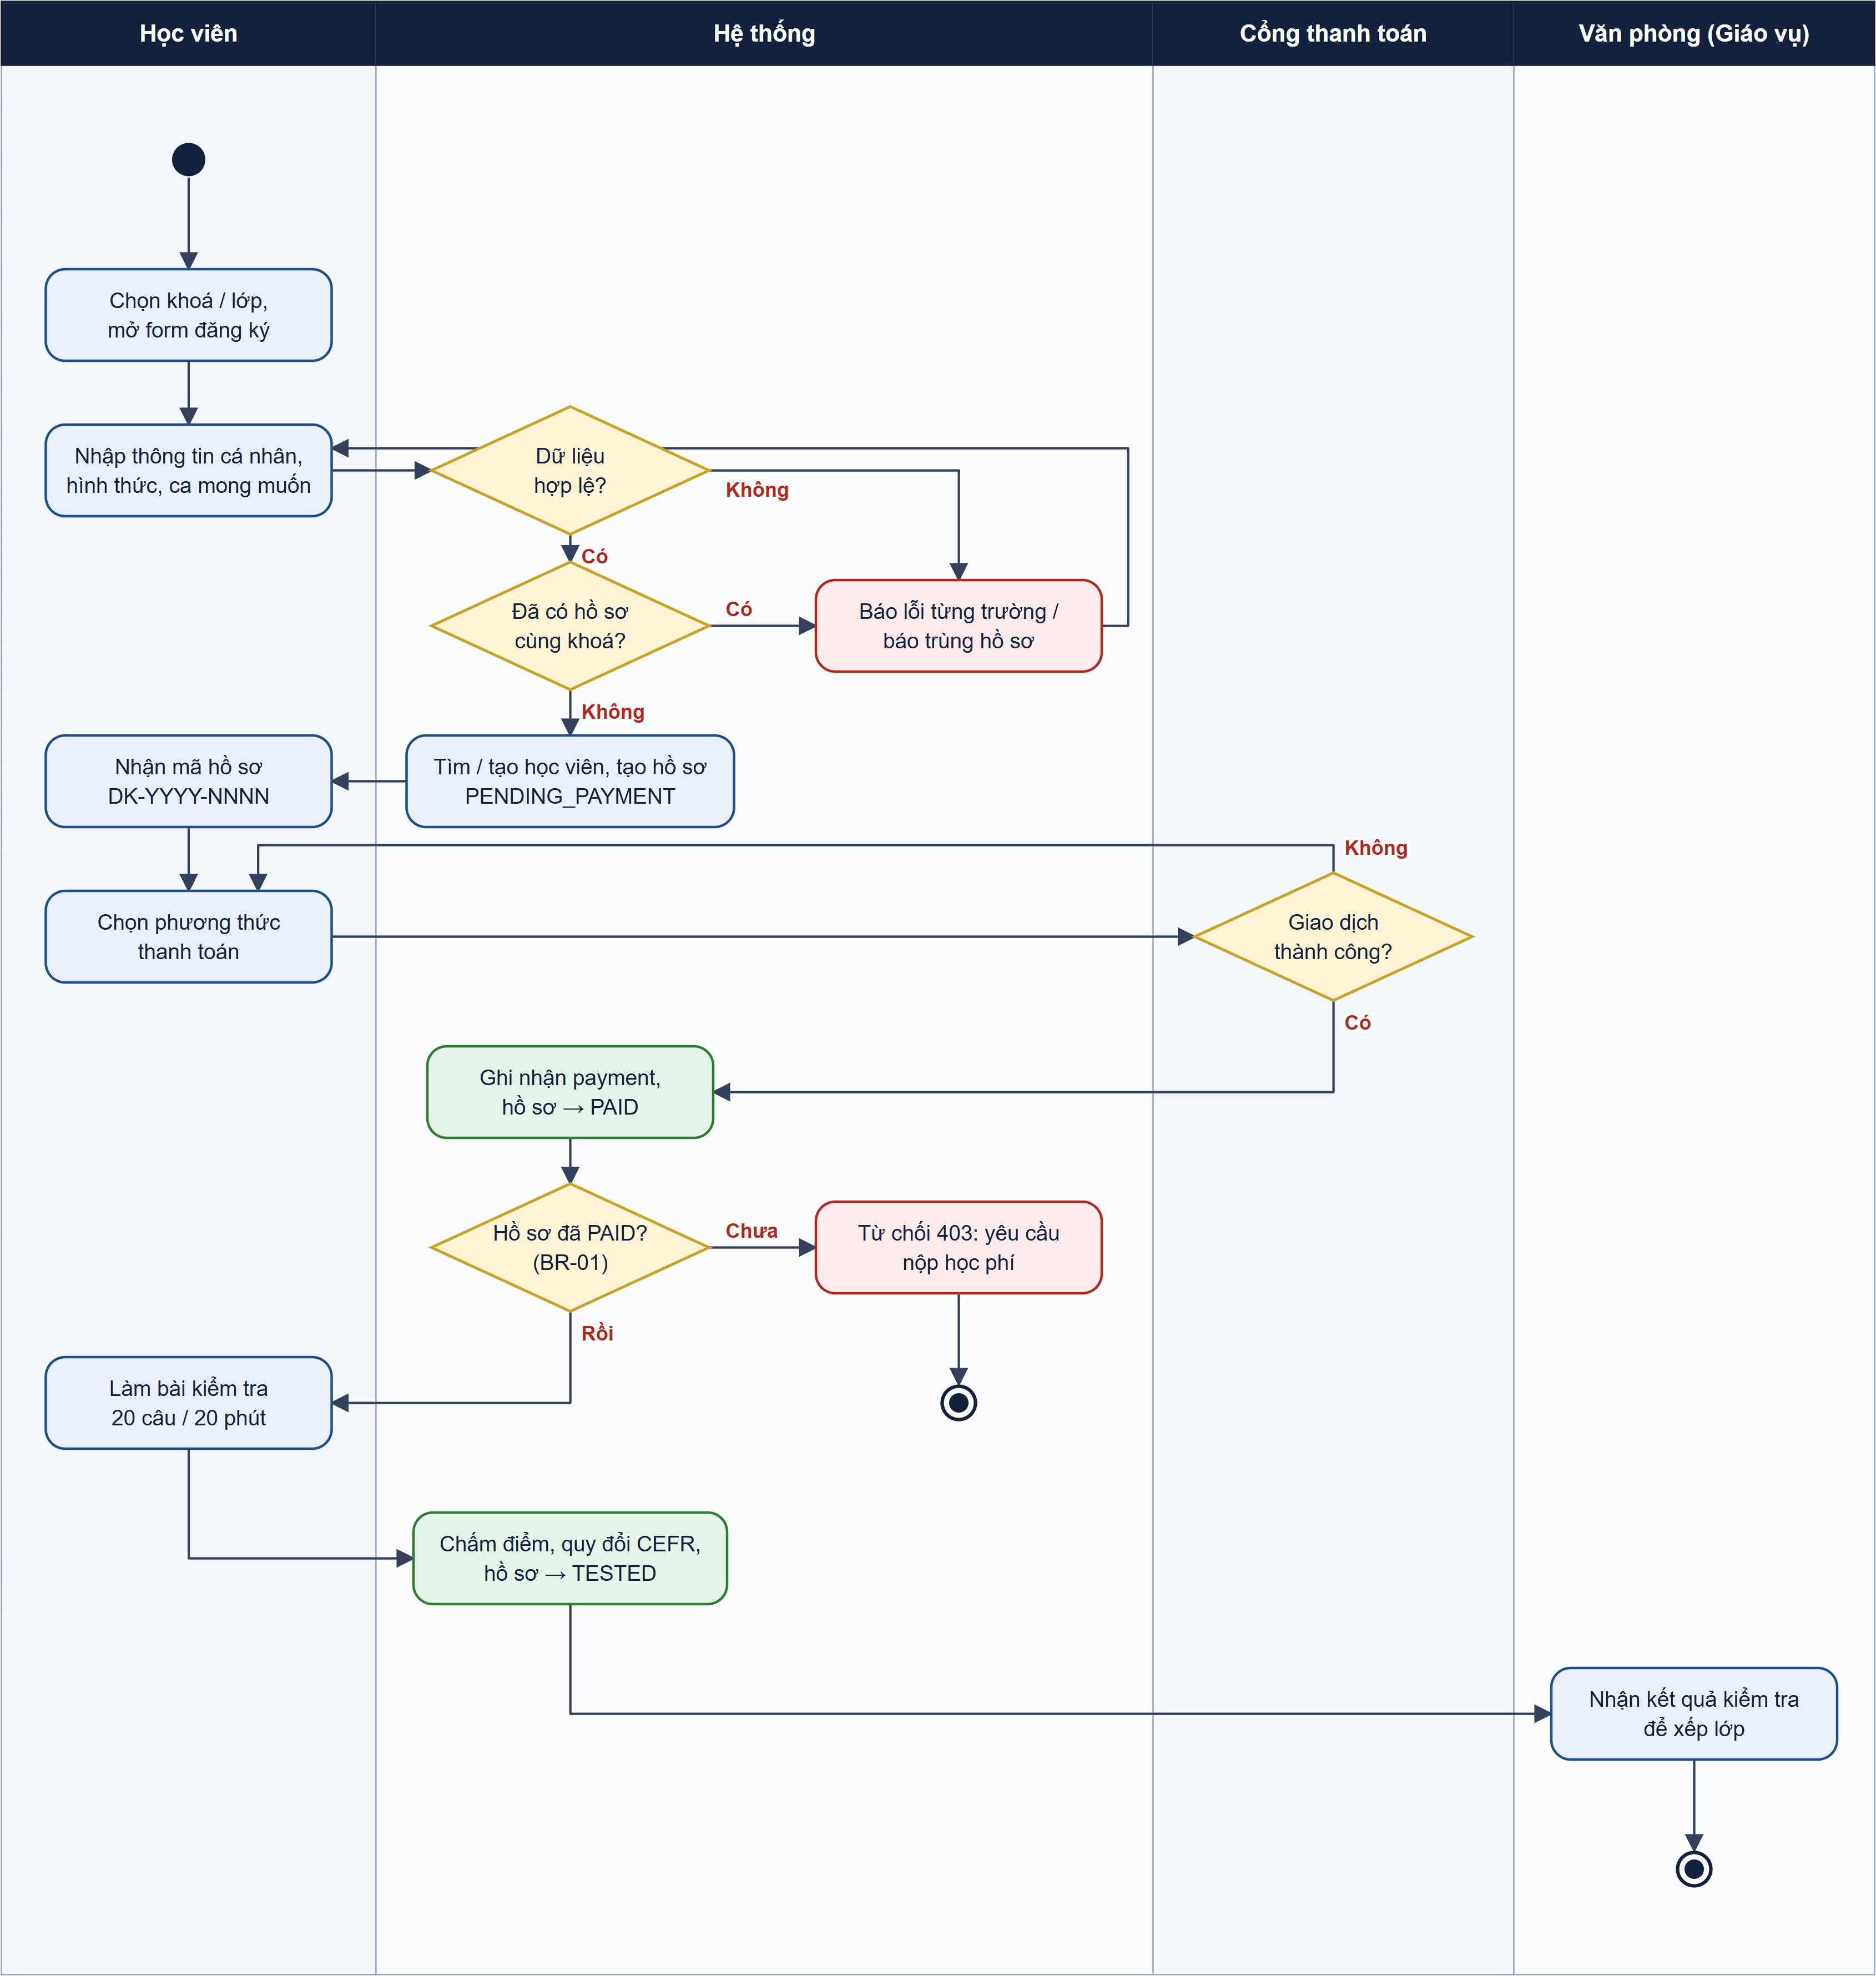
\includegraphics[height=0.82\textheight]{act_01_dangky_thuphi_thi}
    \end{column}
    \begin{column}{0.42\linewidth}
      \begin{itemize}
        \item 4 làn: Học viên, Hệ thống, Cổng thanh toán, Văn phòng
        \item Kiểm tra dữ liệu ở cả trình duyệt và máy chủ
        \item \textbf{BR-01} nằm trong làn hệ thống: gọi thẳng API cũng không thi được khi chưa nộp phí (HTTP 403)
        \item Kết quả CEFR chuyển về văn phòng để xếp lớp
      \end{itemize}
    \end{column}
  \end{columns}
\end{frame}

\begin{frame}{Hoạt động: Xếp lớp và xử lý vượt sĩ số}
  \begin{columns}[c]
    \begin{column}{0.56\linewidth}
      \centering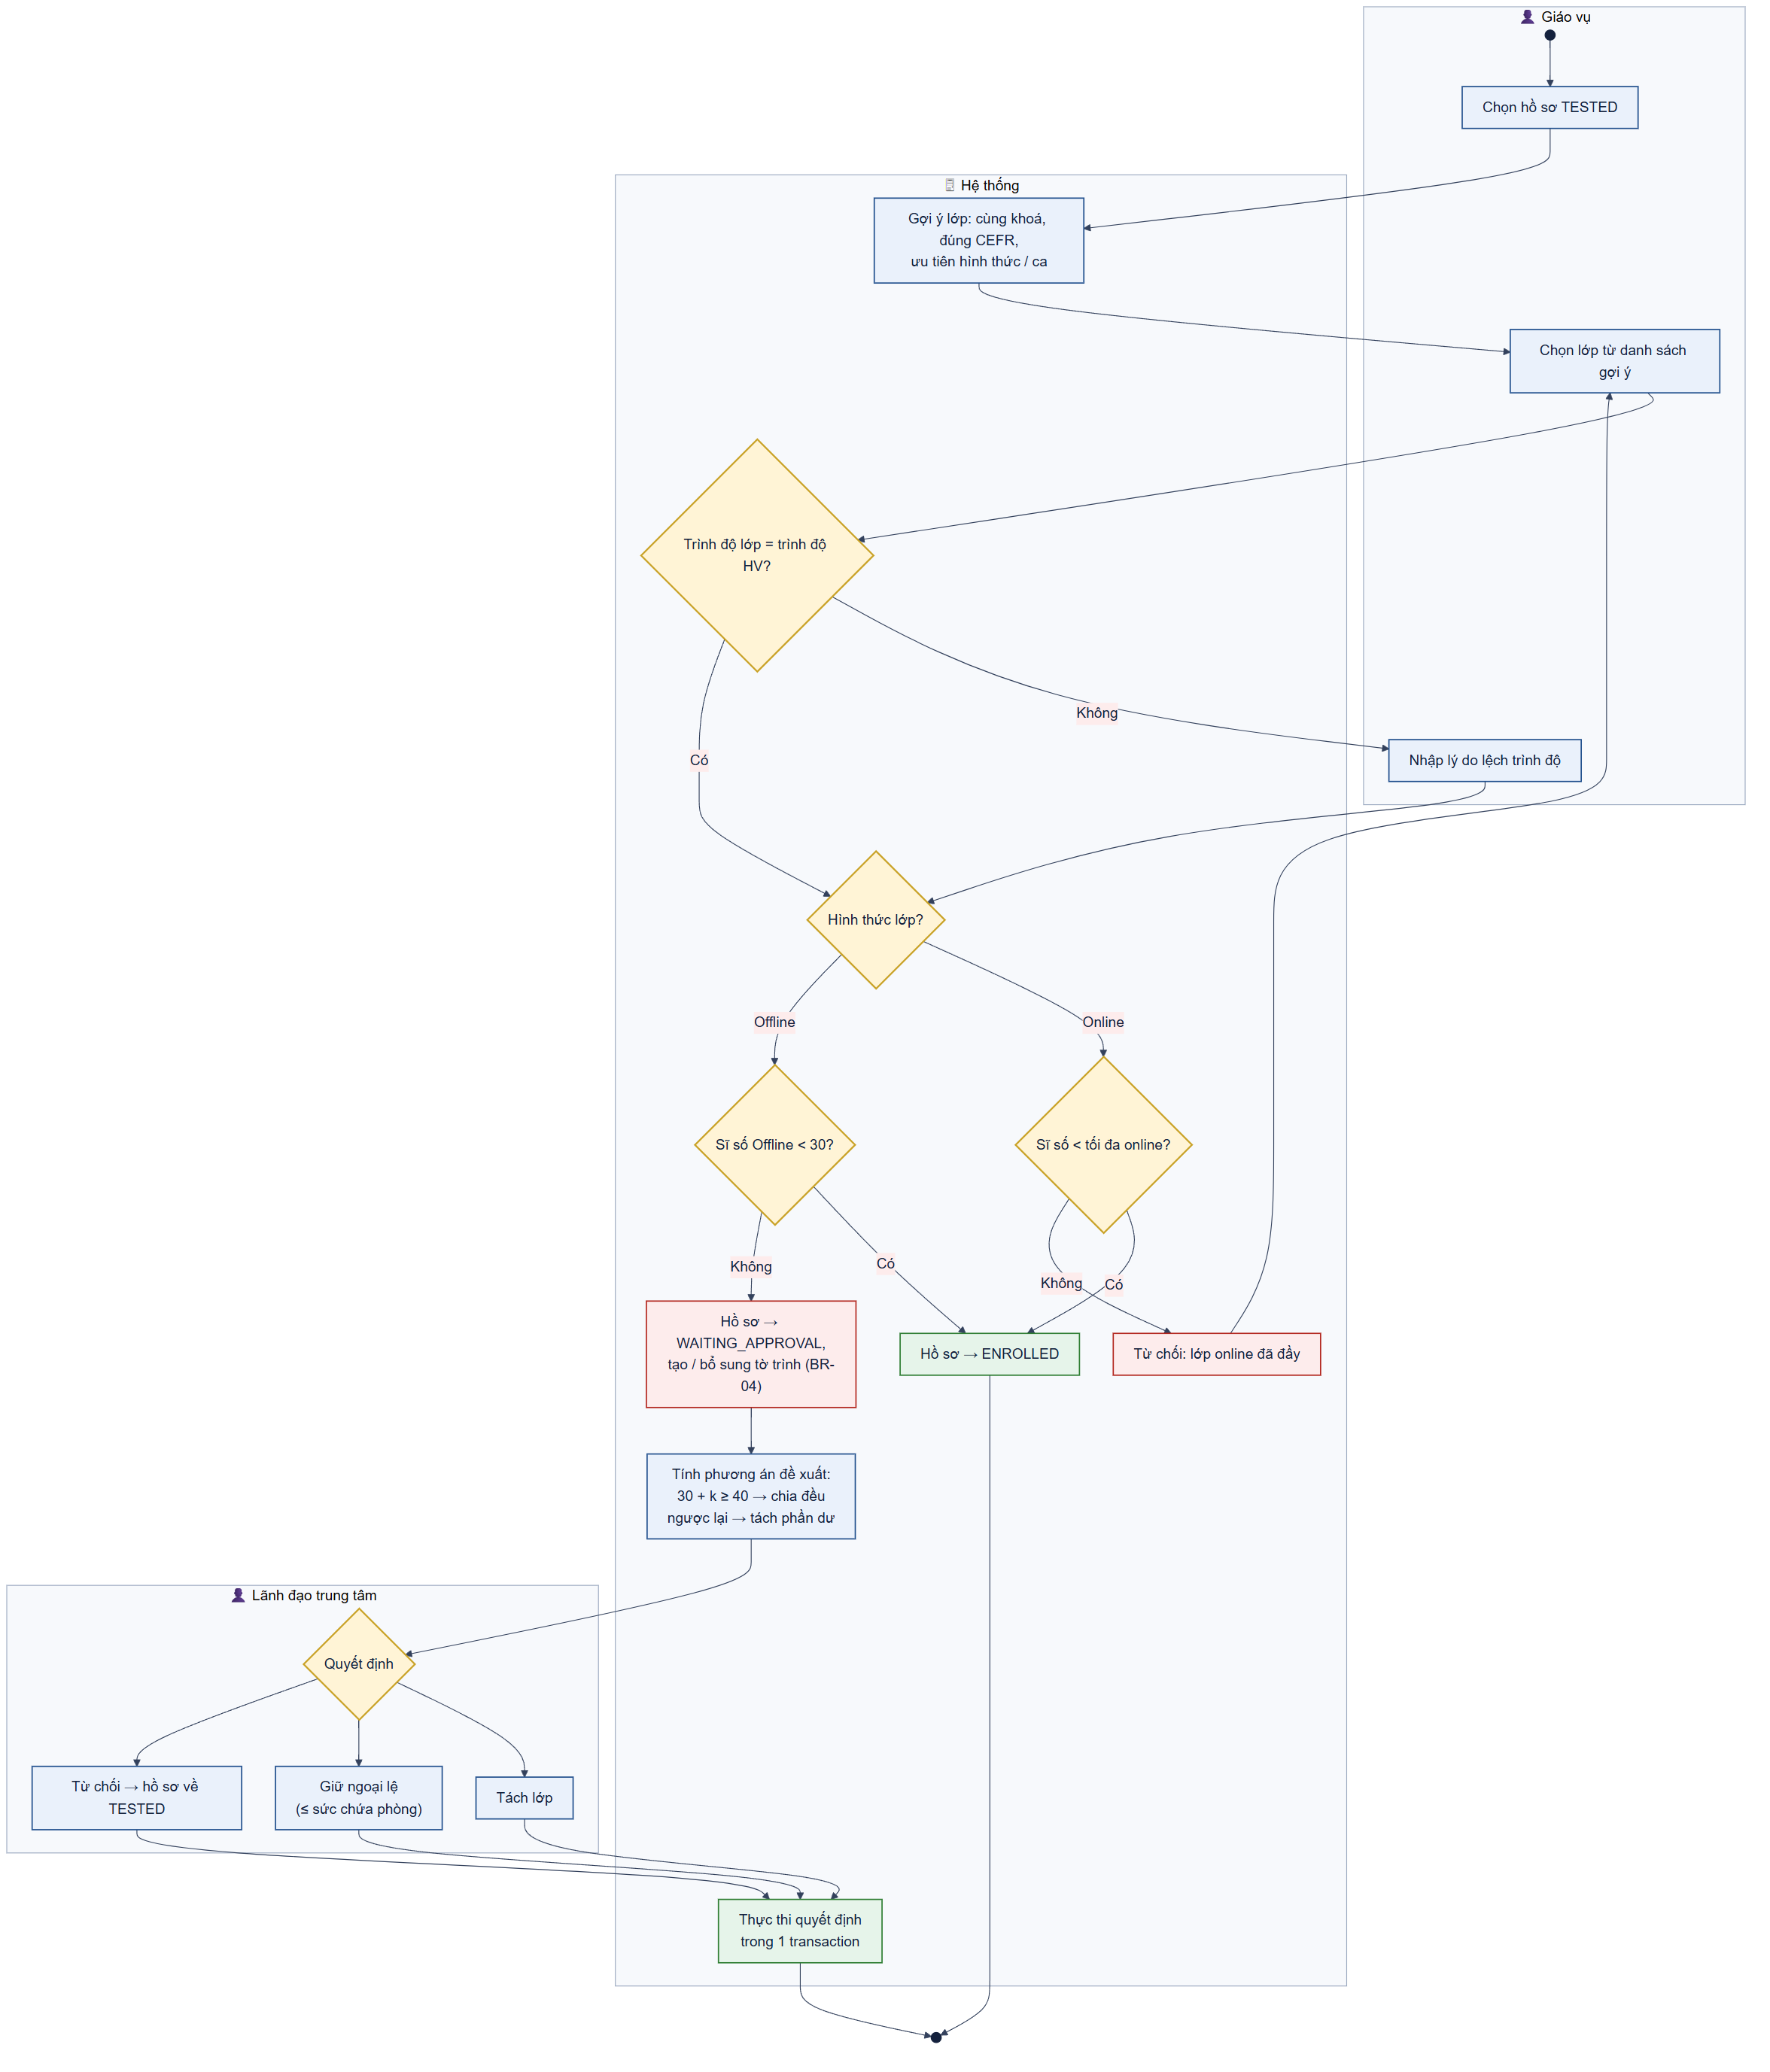
\includegraphics[height=0.82\textheight]{act_02_xeplop_pheduyet}
    \end{column}
    \begin{column}{0.42\linewidth}
      \begin{itemize}
        \item Gợi ý lớp theo trình độ, hình thức, ca học
        \item Xếp lệch trình độ phải ghi lý do
        \item \textbf{Online đầy} → từ chối, chọn lớp khác
        \item \textbf{Offline đủ 30} → hệ thống \alert{không tự xếp}, lập tờ trình
        \item Quyết định của Lãnh đạo được thực thi trong \textbf{một giao dịch}
      \end{itemize}
    \end{column}
  \end{columns}
\end{frame}

\begin{frame}{Vòng đời của Lớp học và Hồ sơ đăng ký}
  \begin{columns}[c]
    \begin{column}{0.27\linewidth}
      \centering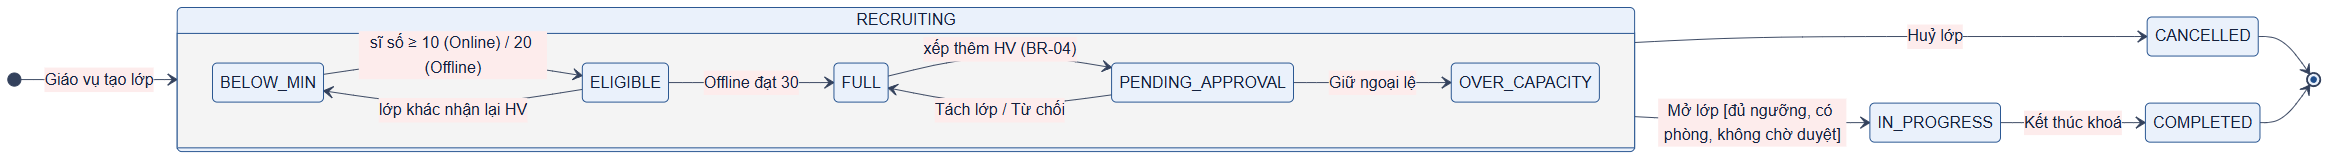
\includegraphics[height=0.80\textheight]{st_01_lop}
    \end{column}
    \begin{column}{0.37\linewidth}
      \centering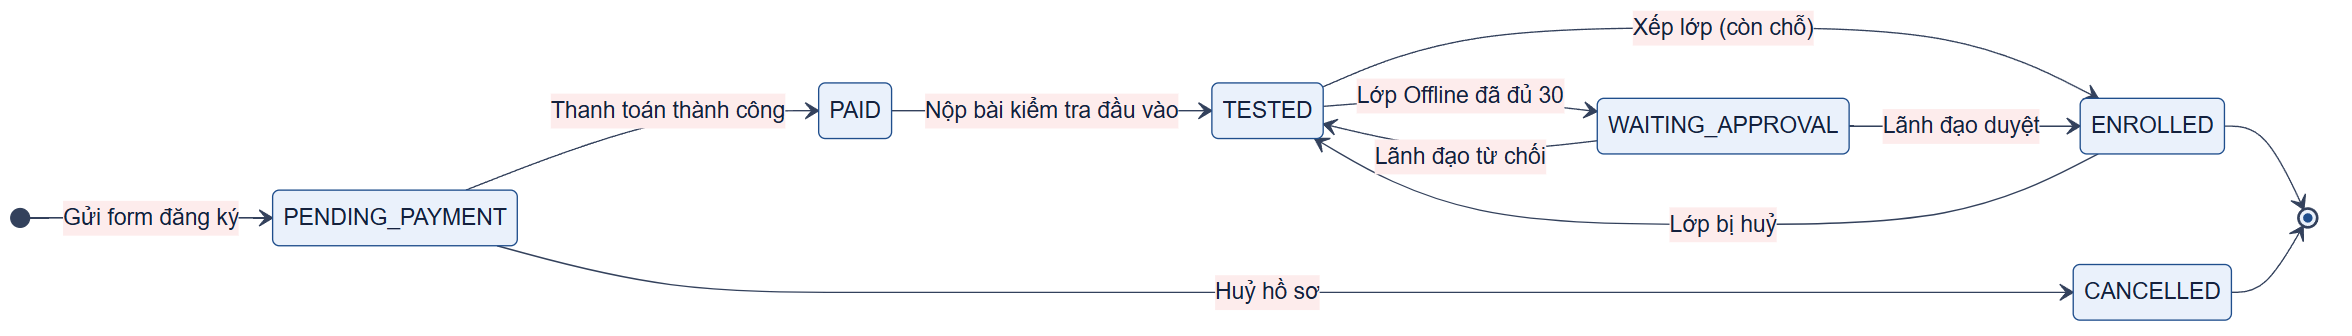
\includegraphics[width=\linewidth]{st_02_hoso}
    \end{column}
    \begin{column}{0.33\linewidth}
      \small
      \textbf{Lớp học} có 2 loại trạng thái:
      \begin{itemize}
        \item \emph{Vòng đời} (lưu CSDL): tuyển sinh → đang học → kết thúc / huỷ
        \item \emph{Sĩ số} (tính toán): chưa đủ, đủ mở, đầy, chờ duyệt, vượt
      \end{itemize}
      \textbf{Hồ sơ:} chờ nộp phí → đã nộp → đã thi → đã xếp lớp (hoặc chờ duyệt sĩ số)
    \end{column}
  \end{columns}
\end{frame}

\begin{frame}{Thiết kế cơ sở dữ liệu}
  \begin{columns}[c]
    \begin{column}{0.5\linewidth}
      \centering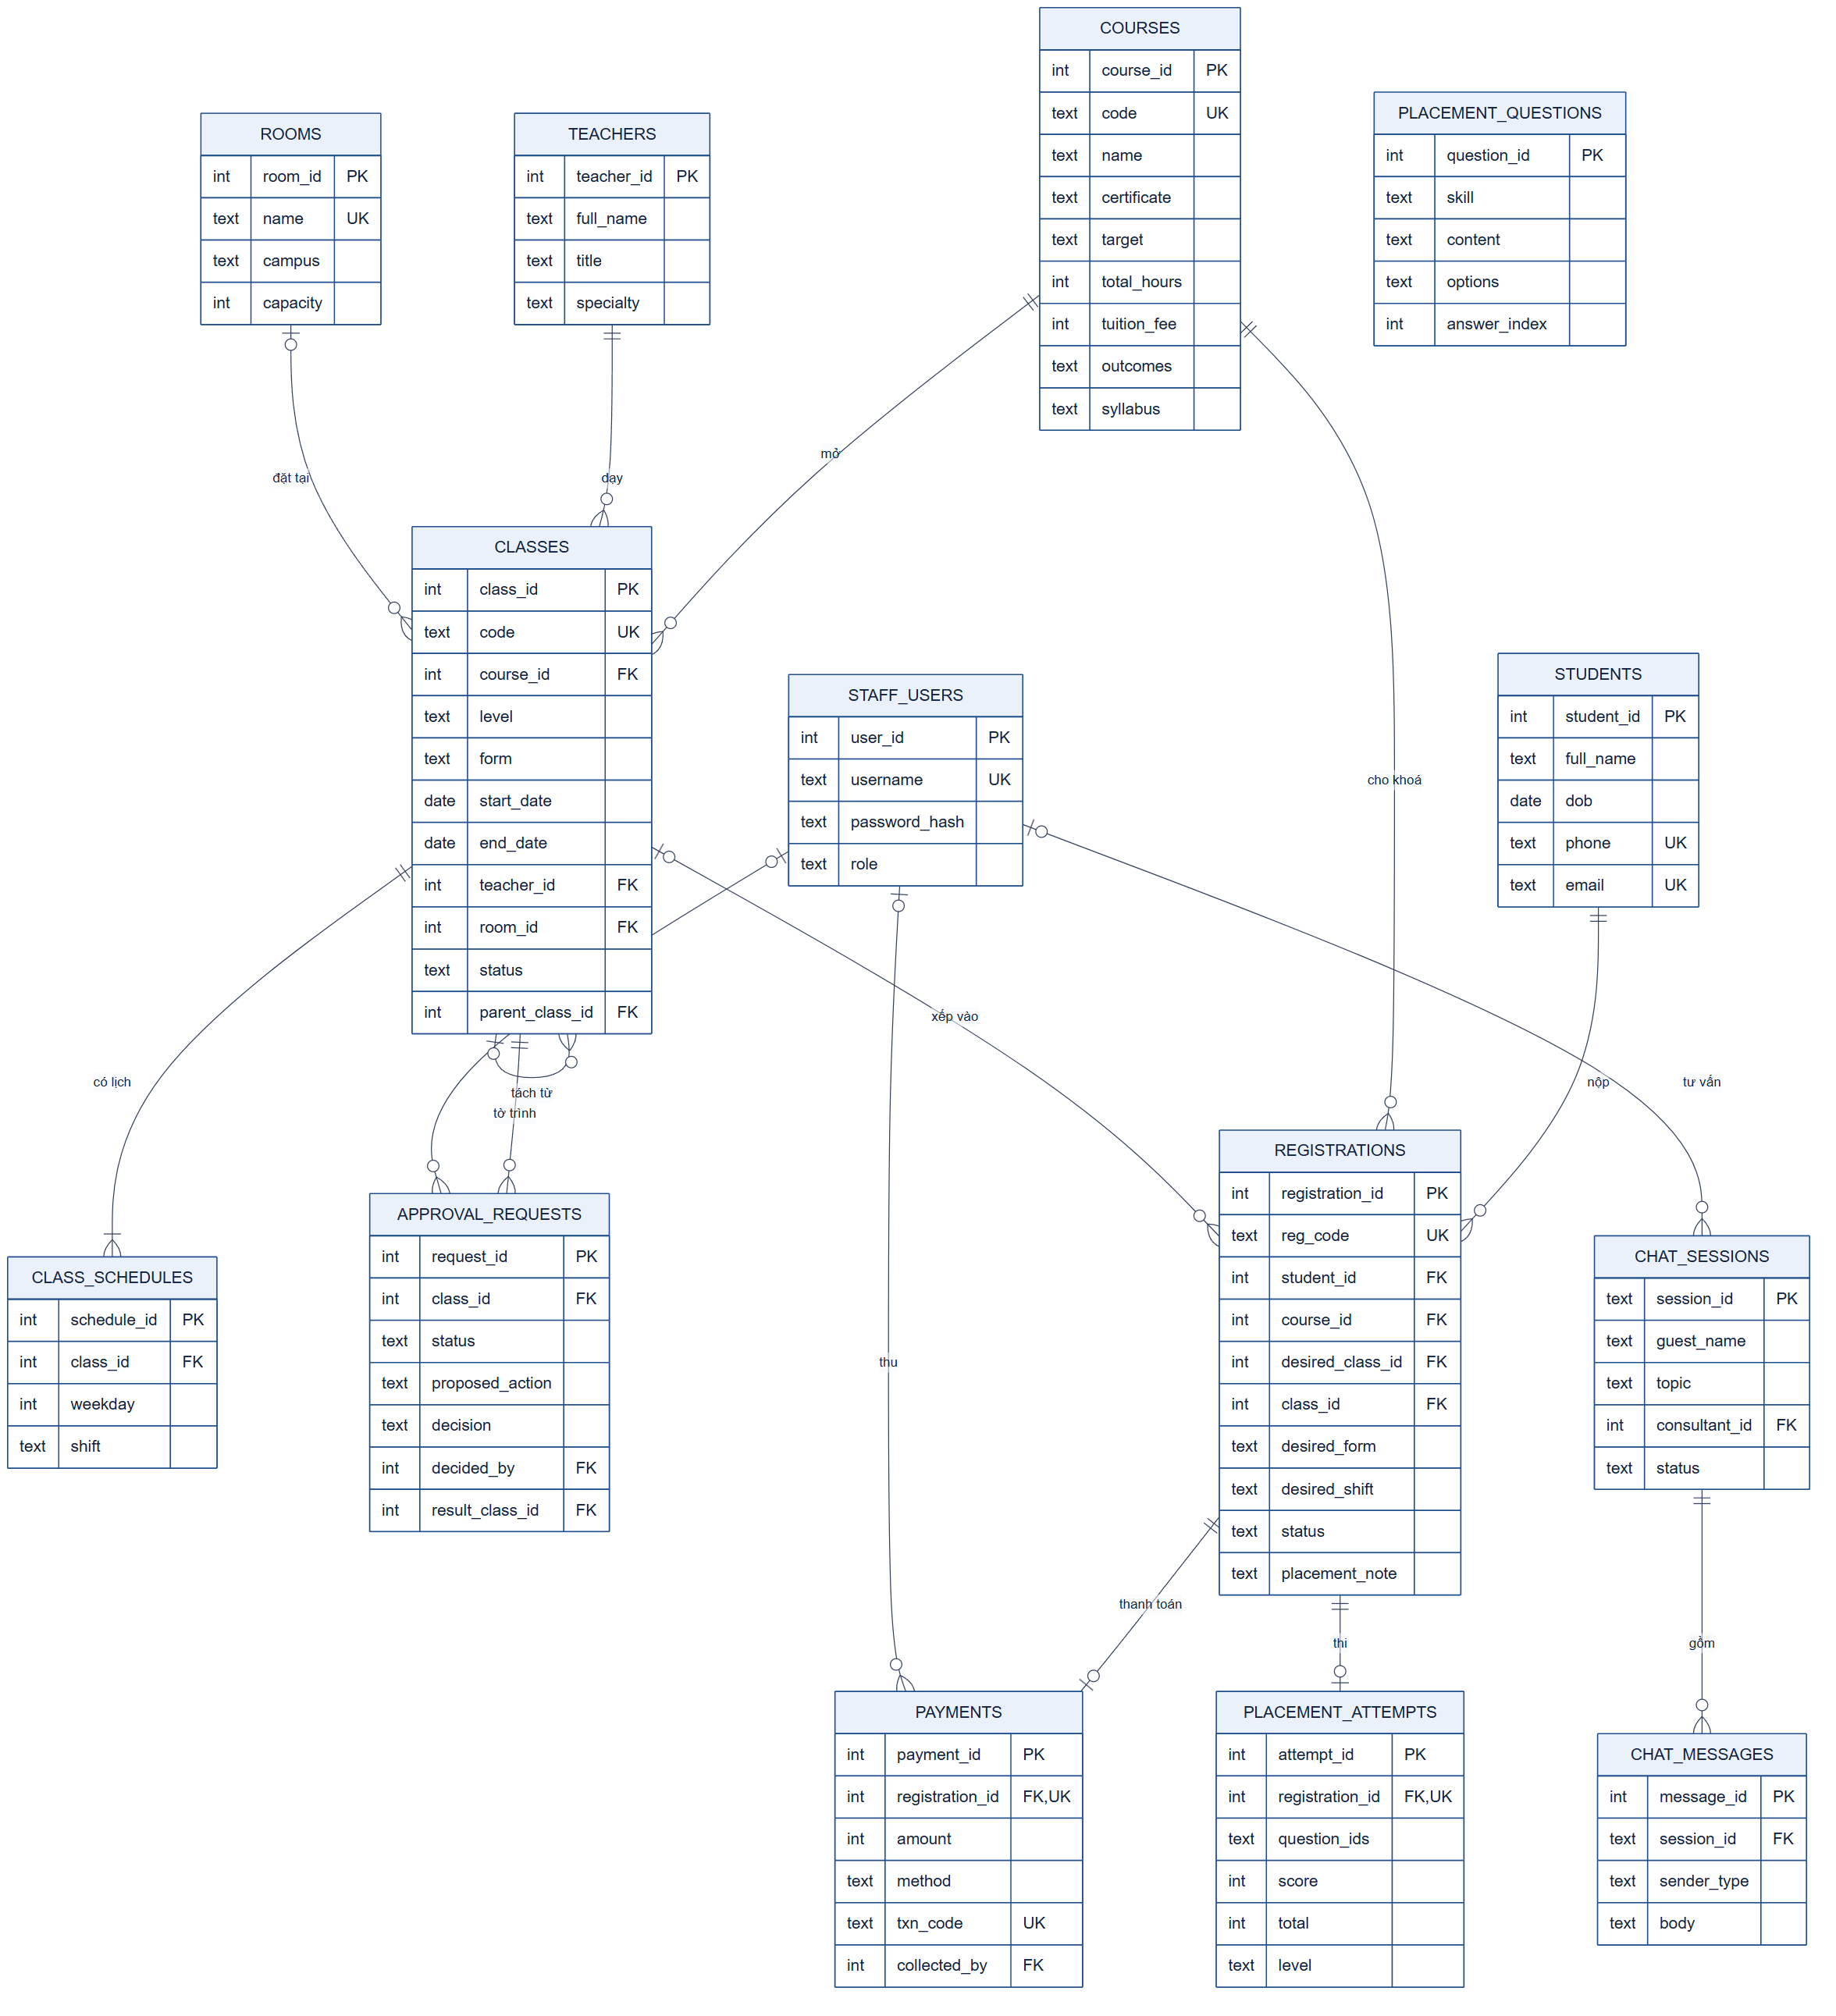
\includegraphics[height=0.82\textheight]{erd_01}
    \end{column}
    \begin{column}{0.48\linewidth}
      \textbf{14 bảng chuẩn 3NF} (SQLite)
      \begin{itemize}
        \item Sĩ số là \textbf{giá trị tính toán} qua view, không lưu bộ đếm → không bao giờ lệch
        \item Ràng buộc nghiệp vụ ngay trong CSDL:
        \begin{itemize}
          \item mỗi lớp tối đa 1 tờ trình đang chờ
          \item mỗi học viên 1 hồ sơ hiệu lực / khoá
          \item hồ sơ có lớp $\Leftrightarrow$ đã xếp hoặc chờ duyệt
          \item lớp online không có phòng
        \end{itemize}
        \item Thao tác nhiều bước chạy trong giao dịch (transaction)
      \end{itemize}
    \end{column}
  \end{columns}
\end{frame}

\begin{frame}{Kiến trúc và công nghệ}
  \centering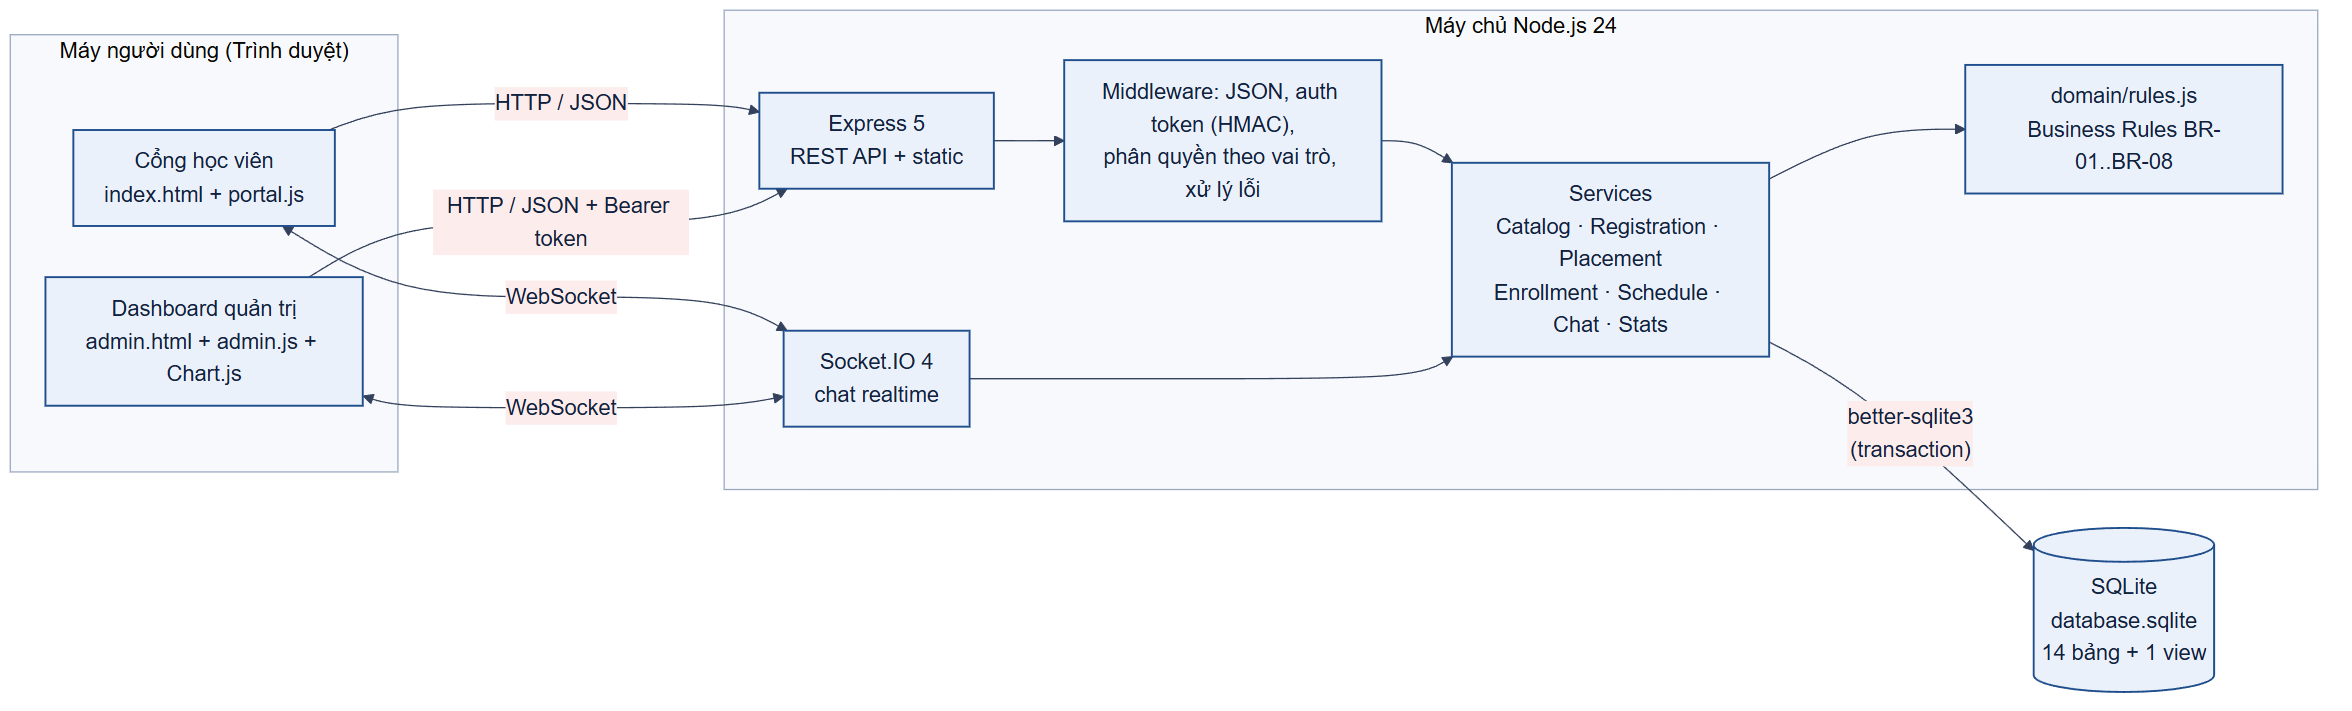
\includegraphics[width=0.86\linewidth]{arch_01}
  \vspace{4pt}
  \small
  \begin{columns}[T]
    \begin{column}{0.32\linewidth}
      \textbf{Máy chủ:} Node.js 24, Express 5\\ \textbf{Realtime:} Socket.IO 4
    \end{column}
    \begin{column}{0.32\linewidth}
      \textbf{CSDL:} SQLite (better-sqlite3)\\ \textbf{Giao diện:} HTML/CSS/JS, Chart.js
    \end{column}
    \begin{column}{0.32\linewidth}
      \textbf{Phân tầng:} routes → services → \alert{rules.js} (hàm thuần chứa quy tắc nghiệp vụ)
    \end{column}
  \end{columns}
\end{frame}

\begin{frame}[fragile]{Quy tắc nghiệp vụ tập trung trong một mô-đun}
\begin{lstlisting}
function placementDecision({ cls, enrolled, registration, studentLevel, reason }) {
  if (registration.status !== 'TESTED')      return { action: 'REJECT', code: 'INVALID_STATUS' };
  if (cls.course_id !== registration.course_id) return { action: 'REJECT', code: 'WRONG_COURSE' };
  if (cls.level !== studentLevel && !reason) return { action: 'REJECT', code: 'LEVEL_MISMATCH' }; // BR-06
  const { max } = limitsOf(cls.form);                        // ONLINE 40 / OFFLINE 30
  if (cls.form === 'ONLINE')
    return enrolled >= max ? { action: 'REJECT', code: 'ONLINE_FULL' }   // BR-02
                           : { action: 'ENROLL' };
  if (enrolled >= max) return { action: 'NEEDS_APPROVAL', code: 'OVER_30' };  // BR-04: không tự xếp
  return { action: 'ENROLL' };
}
\end{lstlisting}
  \vspace{2pt}
  \begin{itemize}
    \item Hàm thuần, không đụng CSDL → kiểm thử từng giá trị biên (29/30/31 học viên…)
    \item Dùng chung cho API, socket và dữ liệu mẫu → một nguồn sự thật duy nhất
  \end{itemize}
\end{frame}

% =====================================================================
\section{Kết quả cài đặt}

\begin{frame}{Chức năng 1 – Quảng bá thông tin lớp học}
  \begin{columns}[c]
    \begin{column}{0.63\linewidth}
      \shot{02_khoa_hoc}
    \end{column}
    \begin{column}{0.35\linewidth}
      \begin{itemize}
        \item 8 khoá học, 4 loại chứng chỉ
        \item Mục tiêu, chuẩn đầu ra, số giờ, học phí
        \item Số lớp Online / Offline đang tuyển, ngày khai giảng gần nhất
        \item Xem lộ trình chi tiết và các lớp đang mở
      \end{itemize}
    \end{column}
  \end{columns}
\end{frame}

\begin{frame}{Chức năng 3 – Tra cứu danh sách lớp}
  \begin{columns}[c]
    \begin{column}{0.63\linewidth}
      \shot{04_tra_cuu_lop}
    \end{column}
    \begin{column}{0.35\linewidth}
      \begin{itemize}
        \item Lọc theo từ khoá, chứng chỉ, hình thức, ca, trình độ, ngày khai giảng, còn chỗ
        \item Kết quả cập nhật tức thì
        \item Thanh sĩ số có \textbf{vạch ngưỡng mở lớp} (10 / 20)
        \item Nhãn trạng thái: chưa đủ, đủ điều kiện mở, chờ Lãnh đạo duyệt
      \end{itemize}
    \end{column}
  \end{columns}
\end{frame}

\begin{frame}{Chức năng 2 – Đăng ký, nộp học phí, kiểm tra đầu vào}
  \begin{columns}[c]
    \begin{column}{0.325\linewidth}\shot{05_dang_ky_validate}\\[2pt] {\scriptsize Form đăng ký, báo lỗi theo từng trường}\end{column}
    \begin{column}{0.325\linewidth}\shot{18_tra_cuu_ho_so_thanh_toan}\\[2pt] {\scriptsize Tra cứu hồ sơ (mã + SĐT), nộp học phí}\end{column}
    \begin{column}{0.325\linewidth}\shot{20_bai_kiem_tra}\\[2pt] {\scriptsize Bài kiểm tra 20 câu – 20 phút}\end{column}
  \end{columns}
  \vspace{8pt}
  \small Hồ sơ đi qua 4 bước: \textbf{Đăng ký → Nộp học phí → Kiểm tra đầu vào → Xếp lớp}. Bài thi chấm tự động, quy đổi CEFR (A1–C1); đáp án không bao giờ gửi về trình duyệt.
\end{frame}

\begin{frame}{Chức năng 4 – Chat room tư vấn thời gian thực}
  \begin{columns}[c]
    \begin{column}{0.49\linewidth}\shot{16_chat_hoc_vien_nhan_tin}\\[2pt] {\scriptsize Phía học viên: widget chat}\end{column}
    \begin{column}{0.49\linewidth}\shot{15_console_tu_van}\\[2pt] {\scriptsize Phía tư vấn viên: hàng đợi và hội thoại}\end{column}
  \end{columns}
  \vspace{6pt}
  \small
  \begin{itemize}
    \item Socket.IO: hàng đợi phiên chờ, chỉ một tư vấn viên nhận được mỗi phiên, báo “đang soạn tin”
    \item Mọi tin nhắn lưu CSDL; tải lại trang vẫn khôi phục phiên và lịch sử
  \end{itemize}
\end{frame}

\begin{frame}{Dashboard văn phòng}
  \begin{columns}[c]
    \begin{column}{0.62\linewidth}
      \shot{08_dashboard}
    \end{column}
    \begin{column}{0.36\linewidth}
      \begin{itemize}
        \item Doanh thu, đăng ký mới, hồ sơ chờ xếp lớp, tờ trình chờ duyệt
        \item Biểu đồ doanh thu – đăng ký 6 tháng
        \item Phễu tuyển sinh: đăng ký → nộp phí → thi → xếp lớp
        \item Sĩ số từng lớp so với ngưỡng
        \item 3 vai trò: tư vấn viên, giáo vụ, lãnh đạo
      \end{itemize}
    \end{column}
  \end{columns}
\end{frame}

\begin{frame}{Xếp lớp và phê duyệt vượt sĩ số}
  \begin{columns}[c]
    \begin{column}{0.49\linewidth}\shot{11_xep_lop}\\[2pt] {\scriptsize Giáo vụ: gợi ý lớp; lớp đủ 30 hiện nút “Lập tờ trình”}\end{column}
    \begin{column}{0.49\linewidth}\shot{14_phe_duyet}\\[2pt] {\scriptsize Lãnh đạo: 3 phương án, hệ thống đánh dấu “Đề xuất”}\end{column}
  \end{columns}
  \vspace{6pt}
  \small Ví dụ trong dữ liệu mẫu: lớp 30 + 3 hồ sơ chờ, phòng 40 chỗ → đề xuất \textbf{giữ ngoại lệ}; lớp 30 + 12 → đề xuất \textbf{chia đều 21 + 21} (phòng 35 chỗ không đủ để giữ).
\end{frame}

% =====================================================================
\section{Kiểm thử và kết luận}

\begin{frame}{Kiểm thử tự động}
  \begin{columns}[T]
    \begin{column}{0.5\linewidth}
      \small
      \begin{tabularx}{\linewidth}{|>{\raggedright\arraybackslash}X|c|c|}
        \hline
        \headrow \hd{Bộ kiểm thử} & \hd{Số ca} & \hd{Đạt} \\ \hline
        Quy tắc nghiệp vụ (đơn vị) & 39 & 39 \\ \hline
        REST API (tích hợp, CSDL tạm) & 31 & 31 \\ \hline
        Chat Socket.IO (thời gian thực) & 8 & 8 \\ \hline
        \textbf{Tổng} & \textbf{78} & \textbf{78 (100\%)} \\ \hline
      \end{tabularx}
      \vspace{8pt}

      Chạy bằng một lệnh \texttt{npm test}, mỗi bộ dùng CSDL riêng nên lặp lại được.
    \end{column}
    \begin{column}{0.47\linewidth}
      \textbf{Tập trung vào giá trị biên và luồng đầu – cuối}
      \begin{itemize}
        \item 9/10 (online), 19/20, 30/31 (offline), 39/40 (chia đều)
        \item Thi khi chưa nộp phí → 403
        \item Học viên thứ 31 → tờ trình; tách 42 → 21 + 21; tách 65 → 3 lớp
        \item Trùng phòng / giảng viên → từ chối
        \item Phân quyền, chống SQL injection, khoá tạm khi dò mật khẩu
        \item Hai tư vấn viên tranh một phiên chat
      \end{itemize}
    \end{column}
  \end{columns}
\end{frame}

\begin{frame}{Kết luận}
  \begin{columns}[T]
    \begin{column}{0.5\linewidth}
      \begin{exampleblock}{Đã làm được}
        \begin{itemize}
          \item Phân tích: 14 FR, 8 BR có mã truy vết
          \item Thiết kế: 21 biểu đồ UML/ERD dạng mã nguồn, CSDL 14 bảng
          \item Ứng dụng web chạy thật: 4 chức năng bắt buộc + thu phí, kiểm tra đầu vào, xếp lớp, phê duyệt, lịch – phòng, dashboard
          \item 78 ca kiểm thử tự động đạt 100\%
        \end{itemize}
      \end{exampleblock}
    \end{column}
    \begin{column}{0.47\linewidth}
      \begin{alertblock}{Hạn chế}
        \begin{itemize}
          \item Cổng thanh toán, email/SMS còn mô phỏng
          \item Chưa có điểm danh, nhập điểm từng buổi
          \item Bài thi mới có trắc nghiệm, 45 câu
        \end{itemize}
      \end{alertblock}
      \begin{block}{Hướng phát triển}
        Tích hợp VNPay/MoMo thật · phân hệ điểm danh – điểm số · bài thi thích ứng có phần nghe · chatbot ngoài giờ
      \end{block}
    \end{column}
  \end{columns}
\end{frame}

\begin{frame}[plain]
  \begin{tikzpicture}[remember picture,overlay]
    \fill[navy] (current page.south west) rectangle (current page.north east);
    \node[text=white,font=\Huge\bfseries] at ([yshift=1.1cm]current page.center) {Em xin cảm ơn cô đã lắng nghe!};
    \fill[hustred] ([xshift=-1.8cm,yshift=0.25cm]current page.center) rectangle ([xshift=1.8cm,yshift=0.33cm]current page.center);
    \node[text=white!85,font=\large] at ([yshift=-0.55cm]current page.center) {Rất mong nhận được nhận xét và câu hỏi của cô};
    \node[text=white!65,font=\small] at ([yshift=-1.9cm]current page.center) {Nguyễn Lê Quân – 20235199 · Mã nguồn: github.com/leekwanreal/ProjectII};
  \end{tikzpicture}
\end{frame}

\end{document}
